
\documentclass[oneside]{diretrizes}            % Imprimir apenas frente
%\documentclass[doubleside]{diretrizes}        % Imprimir frente e verso

% Importações de pacotes
\usepackage[alf, abnt-emphasize=bf, recuo=0cm, abnt-etal-cite=2, abnt-etal-list=0]{abntex2cite}  % Citações padrão ABNT
\usepackage[utf8]{inputenc}                         % Acentuação direta
\usepackage[T1]{fontenc}                            % Codificação da fonte em 8 bits
\usepackage{graphicx}                               % Inserir figuras
\usepackage{amsfonts, amssymb, amsmath}             % Fonte e símbolos matemáticos
\usepackage{booktabs}                               % Comandos para tabelas
\usepackage{verbatim}                               % Texto é interpretado como escrito no documento
\usepackage{multirow, array}                        % Múltiplas linhas e colunas em tabelas
\usepackage{indentfirst}                            % Endenta o primeiro parágrafo de cada seção.
\usepackage{microtype}                              % Para melhorias de justificação?
\usepackage[algoruled, portuguese]{algorithm2e}     % Escrever algoritmos
\usepackage{float}                                  % Utilizado para criação de floats
\usepackage{times}                                  % Usa a fonte Times
\usepackage{xcolor}
\usepackage{color}
\usepackage{tikz}
\usepackage{epic}
\usepackage{multicol}
\usepackage{booktabs}
\usepackage{pdfpages}
\usepackage{subfig}
\usepackage{listingsutf8}
\usepackage{listings}\lstset{
    columns=fullflexible, % para poder copiar código do PDF
    numbers=left, 
    frame=L,
    morekeywords={*,...},
    breaklines=true,
    showstringspaces=false,
    captionpos=b,
    xleftmargin=0pt,
    inputencoding=utf8,
extendedchars=false}
\usepackage{endnotes}
\renewcommand\theendnote{\alph{endnote}}
\renewcommand\makeenmark{\textsuperscript{\theenmark)}}
\renewcommand\enoteformat{\setlength\parindent{12pt}\makebox[0pt][r]{\theenmark. \,}}
\renewcommand\notesname{ }

\usepackage{fancyhdr}
\pagestyle{fancy}
\fancyhf{}
\rhead{Overleaf}
\lhead{Guides and tutorials}
\rfoot{Página \thepage}

% Inclui o preâmbulo do documento
%
% Documento: Preâmbulo
%

\usepackage{helvet}
\renewcommand{\familydefault}{\sfdefault}

\instituicao{Universidade Federal de Mato Grosso}
\abreviatura{UFMT}
\departamento{Faculdade de Economia}
\localapresentacao{Cuiabá - MT}
\programa{Graduação em Ciências Econômicas}
%\modalidade{Subsequente ao Ensino Médio}
\nomeautor{Nome do Aluno}
\titulotb{TITÚLO DA MONOGRAFIA A SER DEFENDIDA}
%\subtitulo{Subtítulo do trabalho}
\anoapresentacao{2020}
\grau{Bacharel em Ciências Econômicas}
\dataapresentacao{2020}
\mesapresentacao{Janeiro}

%Dados Orientador
\orientador{Nome do Orientador}
%\coorientador{Raphael Cunha}
\instOrientador{UFMT}
\departamentoorientador{Faculdade de Economia}
\titulacaoorientador{Prof. Dr.}

%Dados Coorientador
%\coorientador{Nome do Coorientador}
%\instCoorientador{UFMT}
%\departamentocoorientador{Campus Cuiabá}
%\titulacaocoorientador{Prof. Dr.}

%Dados Examinador 1
\nmexamum{Membro da Banca 1}
\instexamum{UFMT}
\departamentoexamum{Campus Cuiabá}
\titulacaoexamum{Prof. Dr.}

%Dados Examinador 2
\nomeexamdois{Membro da Banca 2}
\instexamdois{UFMT}
\departamentoexamdois{Campus Cuiabá}
\titulacaoexamdois{Prof. Dr.}

%Dados Examinador 3
%\nmexamdois{Membro da Banca 3}
%\instexamdois{UFMT}
%\departamentoexamdois{Campus Cuiabá}
%\titulacaoexamdois{Prof. Dr.}


\usepackage[a4paper, top=3.0cm, bottom=2.0cm, left=3.0cm, right=2.0cm]{geometry} %teste margem
%\usepackage{titlesec} %teste margem

\newcommand{\blue}[1]{\textcolor{blue}{#1}} % proposed
\newcommand{\red}[1]{\textcolor{red}{#1}} % to be removed
\newcommand{\green}[1]{\textcolor{green}{#1}} % to be discussed?
\newcommand{\yellow}[1]{\textcolor{yellow}{#1}} % ????
\newcommand{\magenta}[1]{\textcolor{magenta}{#1}} % warning - requires attention


% Define as cores dos links e informações do PDF
\makeatletter
\hypersetup{
    portuguese,
    colorlinks,
    linkcolor=black,
    citecolor=black,
    filecolor=black,
    urlcolor=black,
    breaklinks=true,
    pdftitle={\@title},
    pdfauthor={\@author},
    pdfsubject={\imprimirpreambulo},
    pdfkeywords={abnt, latex, abntex, abntex2}
}
\makeatother

% Redefinição de labels
\renewcommand{\algorithmautorefname}{Algoritmo}
\def\equationautorefname~#1\null{Equa\c c\~ao~(#1)\null}

% Cria o índice remissivo
\makeindex

% Início do documento
\begin{document}

% Retira espaço extra obsoleto entre as frases.
\frenchspacing

% Elementos pré textuais
\pretextual
%
% Documento: Capa
%

\makeatletter
\begin{capa}
	\thispagestyle{empty}%limpa estilo da pagina
	\setlength{\baselineskip}{0.72\baselineskip}
    \begin{center} %Alinhamento centralizado

    \textbf{\expandafter\uppercase\expandafter{\imprimirinstituicao}}\\
	\vspace*{0.25cm}%Espaçamento entre linhas
    \textbf{\expandafter\uppercase\expandafter{\imprimirdepartamento}}\\
    %\textbf{\expandafter\uppercase\expandafter{\imprimirprograma}}\\
	\vspace*{5cm}%Espaçamento entre linhas
	\large\textbf{\expandafter\uppercase\expandafter{\imprimirtitulotb}}\\
	\vspace*{6cm}%Espaçamento entre linhas	
	\small\textbf{\expandafter\uppercase\expandafter{\imprimirnomeautor}}\\
	\vspace*{9.0cm}%%Espaçamento entre linhas
	\large\textbf{\expandafter\expandafter{\imprimirlocalapresentacao\\ \imprimirdataapresentacao}}
	%\small\textbf{\expandafter\uppercase\expandafter{\imprimirdata}}\\
		
	\end{center} %Alinhamento centralizado
\end{capa}
\makeatother

	

                   % Capa
%
% Documento: FOLHA DE ROSTO
%

\makeatletter
\begin{folhaderosto}
	\thispagestyle{empty}%limpa estilo da pagina
	
    \begin{center}
    
		\small\textbf{\expandafter\uppercase\expandafter{\imprimirnomeautor}}\\
		\vspace*{6.2 cm}%Espaço entre linhas
		\normalsize\textbf{\expandafter\uppercase\expandafter{\imprimirtitulotb}}\\
		
    \end{center}
	
	\vspace*{2.35 cm}%Espaçamento entre linhas
		    \large%tamanho da fonte 
    		\hfill%Estica horizontamente  com espaços
	    	\begin{minipage}{8 cm}%Minipagina
	    		\begin{small} %Muda tamanho da fonte
	    		\setlength{\baselineskip}{0.7\baselineskip}
				
		    	{Monografia apresentada ao Programa de {\imprimirprograma }
		    	{\imprimirmodalidade} da {\imprimirinstituicao}{ - }{\imprimirdepartamento},
		    	como parte dos requisitos necessários à obtenção do título de
		    	{\imprimirgrau }.}				
				
				\end{small} %Muda tamanho da fonte
		    \end{minipage}%%Minipagina

		 \vspace*{2.35 cm}%Espaçamento entre linhas   	
		\normalsize{Orientador: {\imprimirtitulacaoorientador }{ }{\imprimirorientador.}\\{
		    	}\\ {\imprimirtitulacaocoorientador }{ }{\imprimircoorientador.}}

		    \vspace*{3.65 cm}%Espaçamento entre linhas
		    
		    \begin{center} %Alinhamento centralizado
		    	\normalsize %Muda tamanho da fonte
	    		\textbf{\imprimirlocalapresentacao \\ \imprimirdataapresentacao}
	    	\end{center}%Alinhamento centralizado

\end{folhaderosto}
\makeatother
             % Folha de rosto
% %
% Documento: Folha Catalográfica
%
% gerar o documento aqui
% https://sistemas.ufmt.br/mfc/


\begin{fichacatalografica}
    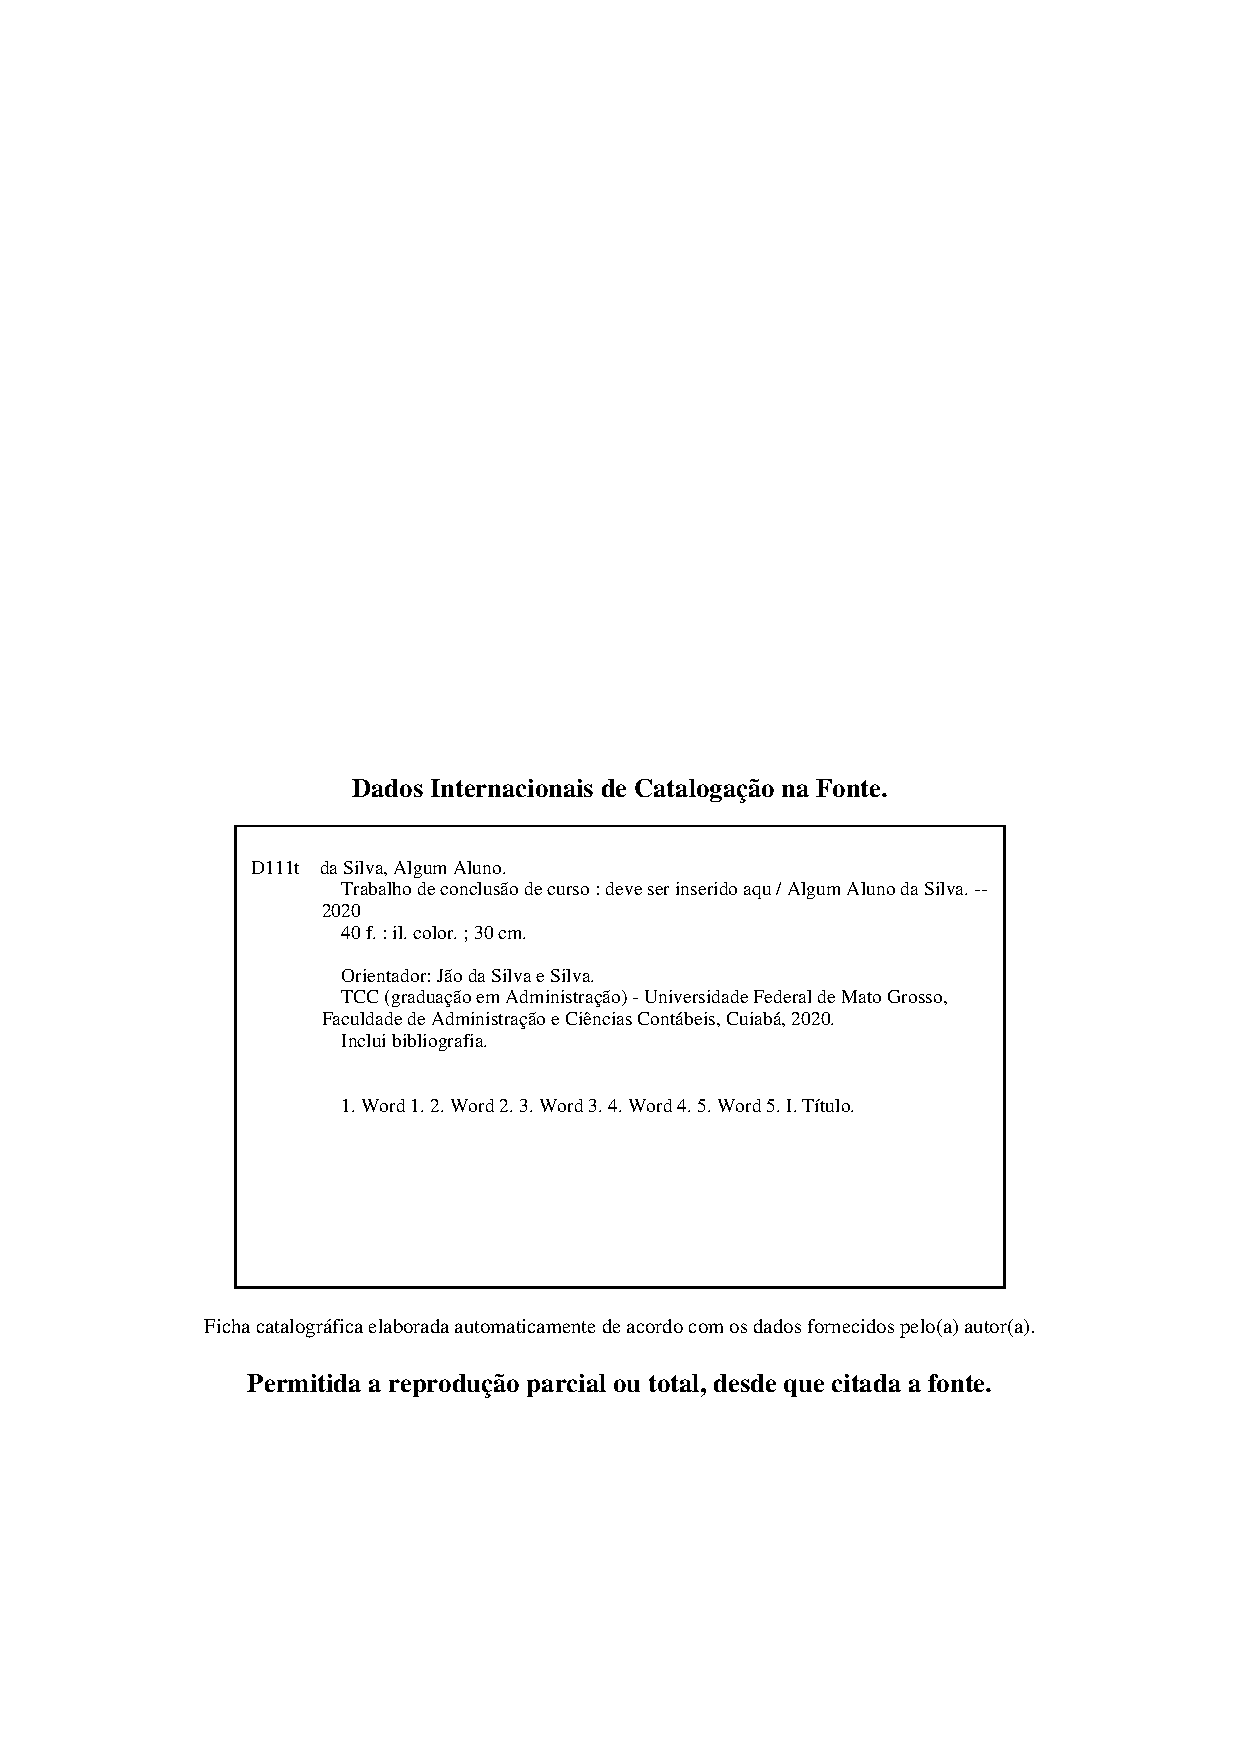
\includepdf[pages=-,pagecommand={\thispagestyle{plain}}]{elementos-pre-textuais/fichaCatalografica.pdf}
\end{fichacatalografica}


    % Gerado pela biblioteca
% %
% Documento: FOLHA APROVAÇÃO
%

\makeatletter
\begin{folhadeaprovacao}

\thispagestyle{empty}%limpa estilo da pagina
	
	\begin{center}
    
		\small\textbf{\expandafter\uppercase\expandafter{\imprimirnomeautor}}\\
		\vspace*{3.0 cm}%Espaço entre linhas
		\normalsize\textbf{\expandafter\uppercase\expandafter{\imprimirtitulotb}}
		
    \end{center}
	
	\vspace*{0.35 cm}%Espaçamento entre linhas
		    \large%tamanho da fonte 
    		\hfill%Estica horizontamente  com espaços
	    	\begin{minipage}{8 cm}%Minipagina
	    		\begin{small} %Muda tamanho da fonte
	    		\setlength{\baselineskip}{0.7\baselineskip}
				
		    	{Monografia apresentada ao Programa de {\imprimirprograma }
		    	{\imprimirmodalidade} da {\imprimirinstituicao}{ - }{\imprimirdepartamento},
		    	como parte dos requisitos necessários à obtenção do título de
		    	{\imprimirgrau }.}\\{
		    	}\vspace*{0.6 cm}\\Orientador:\\ \\
		    	{\imprimirtitulacaoorientador }{ }{\imprimirorientador.}\\{
		    	}\\ %{\imprimirtitulacaocoorientador }{ }{\imprimircoorientador.}			
				
				\end{small} %Muda tamanho da fonte
		    \end{minipage}%%Minipagina
		    	
		    \vspace{0.01 cm}%Espaçamento entre linhas
		    
		    \large%%tamanho da fonte 
    		\hfill%%Estica horizontamente  com espaços
	    	 
		    
		    \normalsize %Muda tamanho da fonte
		    \vspace{0.01 cm}%Espaçamento entre linhas
		    
			\begin{flushleft}%Alinhamento centralizado
			    {Aprovada em {\imprimirmesapresentacao, \imprimiranoapresentacao}.}\\
		 		\textbf{Banca Examinadora}\\ %Negrito
			\end{flushleft}

				\vspace*{0.3 cm}%Espaçamento entre linhas

			\begin{center}	

				\vspace*{0.5 cm}%Espaçamento entre linhas		
				\rule{12 cm}{.1 mm}\\
				{\imprimirtitulacaoorientador}{ }{\imprimirorientador} - Orientador\\
				
				\vspace*{2 cm}%Espaçamento entre linhas
				\rule{12 cm}{.1 mm}\\
				{\imprimirtitulacaoexamum\ \imprimirnmexamum} - {\imprimirinstexamum /\imprimirdepartamentoexamum}
			
				\vspace*{1.5 cm}%Espaçamento entre linhas
				\rule{12 cm}{.1 mm}\\
				{\imprimirtitulacaoexamdois\ \imprimirnomeexamdois} - {\imprimirinstexamdois /\imprimirdepartamentoexamdois}
				
				\vspace*{1 cm}%Espaçamento entre linhas
						
				\vspace*{1.3 cm}%Espaçamento entre linhas
		    \end{center}%Alinhamento centralizado


\end{folhadeaprovacao}
\makeatother
       % Folha de aprovação
% ----------------------------------------------------------
% DEDICATÓRIA
% ----------------------------------------------------------
\begin{dedicatoria}
   \vspace*{\fill}
   \centering
   \noindent
   \textit{ Este trabalho é dedicado a...} \vspace*{\fill}
\end{dedicatoria}

            % Dedicatória
% ----------------------------------------------------------
% AGRADECIMENTOS
% ----------------------------------------------------------
\begin{agradecimentos}

    Agradeço a todos.

\end{agradecimentos}

         % Agradecimentos
% ----------------------------------------------------------
% EPÍGRAFE
% ----------------------------------------------------------
\begin{epigrafe}
    \vspace*{\fill}
	\begin{flushright}
		\textit{``Alguma frase bonita.''\\
		(Autor desconhecido)}
	\end{flushright}
\end{epigrafe}
               % Epígrafe
%
% Documento: Resumo (Português)
%

\begin{RESUMO}
    \thispagestyle{empty}

    \noindent Segundo a \citeonline[3.1-3.2]{NBR6028:2003}, o resumo deve ressaltar o
    objetivo, o método, os resultados e as conclusões do documento. A ordem e a extensão
    destes itens dependem do tipo de resumo (informativo ou indicativo) e do
    tratamento que cada item recebe no documento original. O resumo deve ser
    precedido da referência do documento, com exceção do resumo inserido no
    próprio documento. (\ldots) As palavras-chave devem figurar logo abaixo do
    resumo, antecedidas da expressão Palavras-chave:, separadas entre si por
    ponto e finalizadas também por ponto.

    \vspace*{0.5cm}\noindent\textbf{Palavras-chave}: latex. abntex. editoração de texto.

\end{RESUMO}


% 
% Documento: Resumo (Inglês)
%

\begin{ABSTRACT}
	
		\noindent English text here!

		\vspace*{0.5cm}\noindent\textbf{Keywords}: Word 1, Word 2, Word 3
		
\end{ABSTRACT}
                % Resumo e Abstract
%
% Documento: Lista de figuras
%

\pdfbookmark[0]{\listfigurename}{lof}
\listoffigures*
\cleardoublepage

%
% Documento: Lista de quadros
%

\pdfbookmark[0]{\listofquadrosname}{loq}
\listofquadros*
\cleardoublepage

%
% Documento: Lista de abreviaturas e siglas
%

\begin{siglas}
	\setlength{\baselineskip}{0.7\baselineskip}
	
	\item[IPEA] Instituto de Pesquisa Econômica Aplicada
	\item[RAIS] Relação Anual de Informações Sociais
	\item[WIPO] World Intellectual Property Organization
	\item[OMPI] Organização Mundial da Propriedade Intelectual
	\item[ONU] Organização das Nações Unidas
	\item[ABPI] Associação Brasileira da Propriedade Intelectual
	\item[INPI] Instituto Nacional da Propriedade Industrial 
\end{siglas}

%
% Documento: Lista de tabelas
%

\pdfbookmark[0]{\listtablename}{lot}
\listoftables*
\cleardoublepage
                 % Lista de Figuras, Quadros, Abreviaturas e Tabelas     

\sumario

\begin{OnehalfSpacing}

    % Elementos textuais
    \textual
    %
% Documento: Introdução
%

\chapter{Introdução}

Introdução do trabalho será escrita aqui!
            
    % 
% Resultados encontrados 
% 

\chapter{Análise dos resultados}

Os resultados encontrados foram...

    %
% Conclusão
%

\chapter{Conclusão}

Concluo que...


\end{OnehalfSpacing}

% Elementos pós textuais
\postextual

\bibliography{referencias}       % Referências

\begin{OnehalfSpacing}
    %
% Documento: Apêndices
%

\begin{apendicesenv}

\chapter*{Apêndice A}

Algum conteúdo.

\end{apendicesenv}

\begin{apendicesenv}

\chapter*{Apêndice B}

algum conteúdo.

\end{apendicesenv}
         % Apêndices
    %
% Documento: Anexos
%

\begin{anexosenv}

\chapter{Como elaborar}

Anexo é texto ou documento não elaborado pelo autor, que serve de fundamentação, comprovação e ilustração. Elemento opcional. Deve ser precedido da palavra ANEXO, identifi-cado por letras maiúsculas consecutivas, travessão e pelo respectivo título. Utilizam-se letras maiúsculas dobradas, na identificação dos anexos, quando esgotadas as letras do alfabeto.


\end{anexosenv}            % Anexos
\end{OnehalfSpacing}

\printindex                                             % Índice remissivo

\end{document}
